\documentclass[a4paper,12pt]{article}
\usepackage[top=.5in, nohead, nofoot]{geometry}
\usepackage[latin1]{inputenc}
\usepackage[T1]{fontenc}
\usepackage[dvips]{graphicx}
\usepackage{appendix}
\usepackage{graphics}
\usepackage{amsmath, amsthm,natbib}
\usepackage{amssymb, latexsym}
\usepackage{textcomp}
\usepackage{verbatim}
\usepackage{setspace}
\usepackage{graphics}
\usepackage{wasysym}
\usepackage{float}
\usepackage{color}
\usepackage{rotating}
\usepackage{verbatim}
\usepackage{listings}
\author{C\'oil\'in Minto}
\title{F-B phase plane ideas}
\date{12/11/08}

\begin{document}
%\select@language{english}
\maketitle
\begin{abstract}
The aim of this brief document is to discuss some ideas for the analysis of the relationship between fishing mortality and biomass. The overarching goal is to present graphical and analytical methods to assess whether fishing is the dominant driver of the biomass dynamics for the population. In the process, probabilistic methods are explored for how likely a population is to recover from a depleted state. Methods for exploratory data analysis include: timeseries plots borrowed from meteorology, phase-diagrams, and rose-diagrams. These are accompanied by confirmatory data analysis including Markov transition equations and state space methods for the analysis of movement. These are compared and critiqued.
\end{abstract}
\section{Markov transition probabilities}
Figure~\ref{fig:simplified_pp} shows a hypothetically simplified trajectory in the fishing mortality-biomass phase plane. The plane is divided up into four states $\left\{ {1, 2, 3, 4} \right\}$ denoted by $i$. At a given timestep $t$ there are four possible state transitions for time $t+1$. There are  a total of $4\times 4$ possible transitions, denoted by $X_t$. Let $N_{x_{t+1}|x_{t}}$ denote the number of times a given transition was observed e.g. $N_{2|1}$ is the number of times the transition from state 1 to state 2 was observed. The row totals  denote the sum of the number of movements to that state, as in \\

\hspace{.5in} \begin{tabular}{p{2cm} l | p{1cm}  p{1cm}  p{1cm}  p{1cm} r}
& \multicolumn{4}{r}{time $t$} \\
  &  & 1 & 2 & 3 & 4 & \\
\cline{2-6}
& 1 & $N_{1|1}$  & $N_{1|2}$  &  . & . & {\footnotesize $\displaystyle{\sum_{i=1}^4} N_{1|x_{t}=i}$ }\\
time $t+1$ & 2 &  $N_{2|1}$ & $N_{2|2}$ &  &   & {\footnotesize $\displaystyle{\sum_{i=1}^4} N_{2|x_{t}=i}$} \\
 & 3 & .  &   & .  &  & {\footnotesize $\displaystyle{\sum_{i=1}^4} N_{3|x_{t}=i}$}\\
 & 4 &  . &   &   & .& {\footnotesize $\displaystyle{\sum_{i=1}^4} N_{4|x_{t}=i}$}
\end{tabular}\\

A Markov property holds when 
\begin{equation}
 P(X_{t+1}=x|X_{t}=x_{t},\ldots,X_{1}=x_{1})= P(X_{t+1}=x|X_{t}=x_{t})
\end{equation}
that is, the probability of $X$ being in a given state is solely dependent on the previous time step (WORK ON THIS!).
 \begin{equation}
P(X_{t+1}=x|X_{t}=x_{t})=N_{x_{t+1}|x_{t}}/\displaystyle{\sum_{i=1}^4} N_{x_{t+1}|x_{t}=i}
  \end{equation}
% \end{equation}

\begin{figure}
\begin{center}
 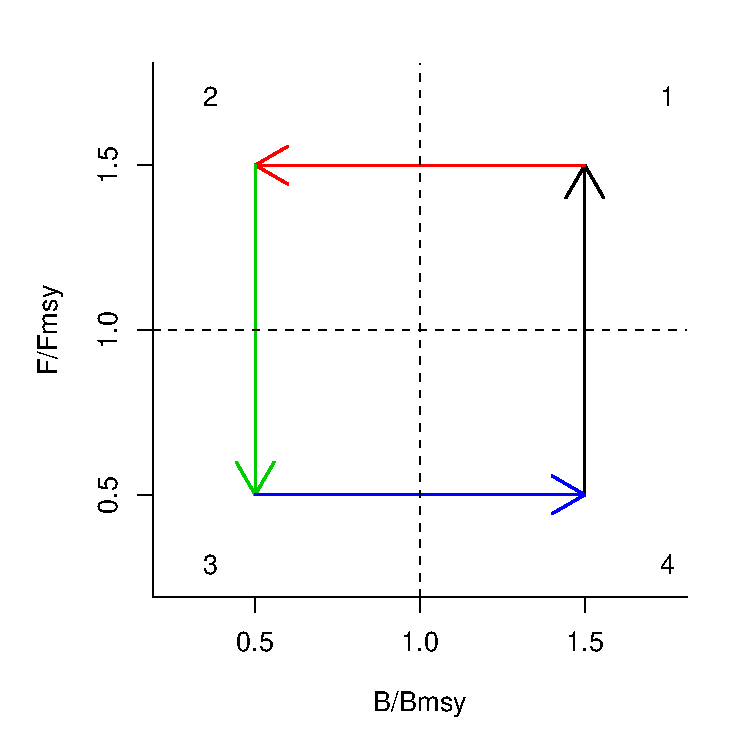
\includegraphics[width=4.5in]{/home/srdbadmin/SQLpg/srdb/trunk/projects/recovery/phase_plane/tex/figures/2_pp_simplified.pdf}	
\caption{Hypothetical simplified phase-plane diagram}
\end{center}
\label{fig:simplified_pp}
\end{figure} 

\end{document}

\section{Schaefer model and the phase-plane}
To investigate possible analyses, population-level data are simulated and then analyzed as if the underlying dynamics were not known. For now, the data are simulated according to a deterministic Schaefer population model given by
\begin{equation}	
 B_{t}=B_{t-1}+r B_{t-1} \left(1-\frac{B_{t-1}}{k}\right)-C_{t-1}
\end{equation}
where $B_{t}$ is the biomass at time $t$ (years), r is the intrinsic discrete rate of population growth, $k$ is the carrying capacity and $C_t$ is the catch. The catch is given by $C_t=F_t B_t$, where $F_t$ is fishing mortality. Can we say that $F_t=qE_t$, where $q$ is catchability and $E_t$ is effort?\\ 
This model ignores population structure but might be useful as a first pass. Appendix~\ref{app:r-code} presents R code to simulate fishing mortality (F) and biomass (B) data. 
% ignores population stage or age structure, migration

% include equations
The resulting deterministic timeseries and phase plane are plotted in Figure~\ref{fig:simFSSB}.
\begin{figure}
\begin{center}
 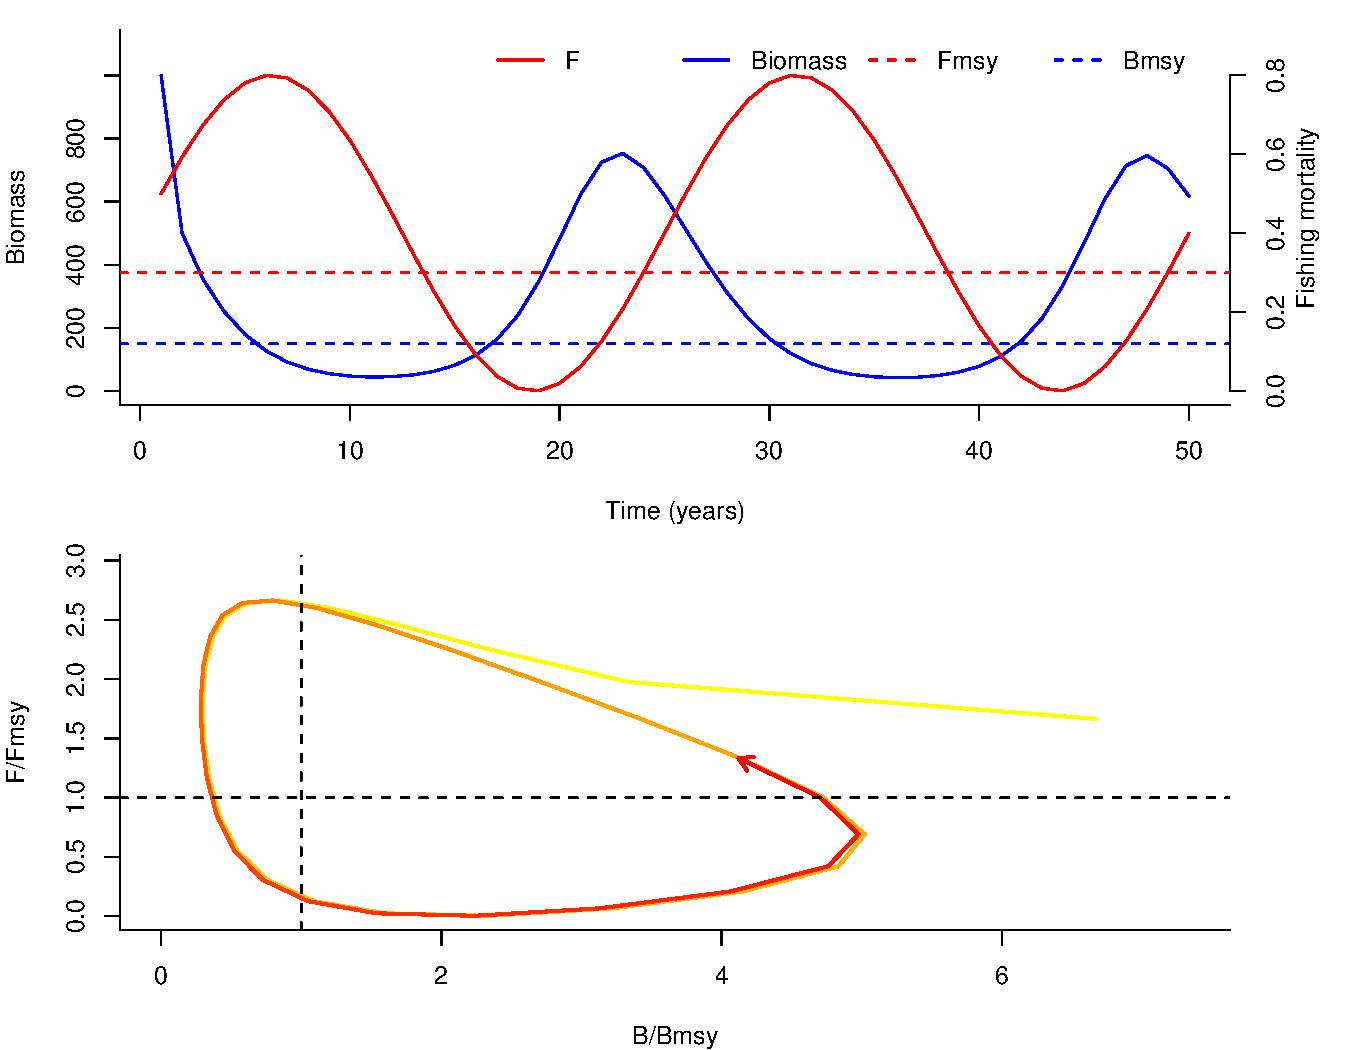
\includegraphics[width=6in]{/home/srdbadmin/SQLpg/srDB/projects/recovery/phase_plane/tex/figures/1_simulated_f_b.pdf}	
\caption{Simulated data assuming Schaefer/logistic population growth with catch. The timeseries are shown in the top panel along with absolute reference points. The resulting scaled phase plane is shown in the bottom panel with 1:1 F=Fmsy and SSB=Bmsy reference points drawn.}
\end{center}
\label{fig:simFSSB}
\end{figure} 

\appendix
\appendixpage
\section{R code}\label{app:r-code}
\subsection{Schaefer model simulation}
\lstset{language=R, breaklines=true}
\lstinputlisting{/home/srdbadmin/SQLpg/srDB/projects/recovery/phase_plane/R/1_simulate_f_tb.R}

\end{document}
\subsection{Additional R functions}
\lstset{language=R, breaklines=true}
\lstinputlisting{/home/srdbadmin/SQLpg/srDB/projects/recovery/phase_plane/R/functions}

